\documentclass{article}
\usepackage{amsmath}
\usepackage{amssymb}
\usepackage[a4paper, top=25mm, bottom=25mm, left=25mm, right=25mm]{geometry}
\usepackage{pgfplots}
\usepackage{mathtools}
\usepgfplotslibrary{fillbetween}
\pgfplotsset{compat=1.18}

\begin{document}
\pagestyle{empty}
\large

\begin{center}
2022-2023 Fall \\MAT123-02,05 Final\\(13/01/2023)
\end{center}

\noindent 1. Evaluate the following definite integrals.

\hfill

\noindent (a) $\displaystyle\int_0^1\frac{x^2}{\sqrt{4-x^2}}\,dx$ \ \ \ (b) $\displaystyle\int_0^{\pi/4}x\sec^2x\,dx$

\hfill

\noindent 2.

\hfill

\noindent (a) Consider the finite region between the curves $y=\mathrm{e}^{-x},\:y=x/\mathrm{e}$, and the $y$-axis. Write a definite integral (do not evaluate) by using the Cylindrical Shell Method, which gives the volume of the solid obtained by rotating this region about the $x$-axis.

\hfill

\noindent (b) Consider the infinite region between the curves $y=\mathrm{e}^{-x},\:y=x/\mathrm{e}$ and the $x$-axis. Write a definite integral (do not evaluate) by using the Washer Method, which gives the volume of the solid obtained by rotating this region about the line $y=-1$.

\hfill

\noindent (c) Evaluate the area of the region given in part (a).

\hfill

\noindent 3. Determine whether each series is convergent or divergent.

\hfill

\noindent (a) $\displaystyle\sum_{n=1}^\infty\frac1{\arctan\left(n^2\right)}$ \ \ \ (b) $\displaystyle\sum_{n=1}^\infty\sin\left(\frac1{n^3}\right)$ \ \ \ (c) $\displaystyle\sum_{n=1}^\infty n\mathrm{e}^{-n^2}$

\hfill

\noindent 4.

\hfill

\noindent (a) Find the radius and interval of convergence of the power series

\[\sum_{n=1}^\infty\frac{2^{n+1}\cdot(x+1)^n}{n\cdot3^n}.\]

\hfill

\noindent (b) Using the formula $\displaystyle\frac1{1-x}=\sum_{n=0}^\infty x^n$ for $\left|x\right|<1$, find the Maclaurin series of the function $\displaystyle f(x)=\frac{x^{123}}{1+x^4}$.

\newpage

\begin{center}
2022-2023 Final (13/01/2023) Solutions\\
(Last update: 8/20/25 (20th of August) 4:38 PM)
\end{center}

\noindent 1.

\hfill

\noindent (a) Let $x=2\sin u$ for $\displaystyle-\frac\pi2<u<\frac\pi2$, then $dx=2\cos u\,du$.

\[x=0\implies2\sin u=0\implies u=0\]

\[x=1\implies2\sin u=1\implies\sin u=\frac12\implies u=\arcsin\frac12=\frac\pi6\]

\begin{align*}
\mathrm{I}&=\int_0^1\frac{x^2}{\sqrt{4-x^2}}\,dx=\int_0^{\pi/6}\frac{4\sin^2u}{\sqrt{4-4\sin^2u}}\cdot2\cos u\,du\int_0^{\pi/6}\frac{4\sin^2u\cos u}{\left|\cos u\right|}\,du\quad\left[\cos u>0\right]\\\\&=\int_0^{\pi/6}4\sin^2u\,du=4\int_0^{\pi/6}\left(1-\cos^2u\right)\,du=4\int_0^{\pi/6}\frac{1-\cos2u}2\,du\\\\&=4\left(\frac u2-\frac{\sin 2u}4\right)\Bigg|_0^{\pi/6}=2u-\sin 2u\:\Bigg|_0^{\pi/6}=\left(\frac\pi3-\sin\frac\pi3\right)-0=\boxed{\frac\pi3-\frac{\sqrt3}2}
\end{align*}

\hfill

\noindent (b) Use the method of integration by parts.

\[\left.\begin{array}{c}
u=x\implies du=dx\\[1em]
dv=\sec^2x\,dx\implies\displaystyle v=\tan x
\end{array}\right\}\rightarrow\int_a^b u\,dv=uv\bigg|_a^b-\int_a^b v\,du\]

\begin{align*}\int_0^{\pi/4} x\sec^2x\,dx&=x\tan x\bigg|_0^{\pi/4}-\int_0^{\pi/4}\tan x\,dx=x\tan x+\ln\left|\cos x\right|\bigg|_0^{\pi/4}=\boxed{\frac\pi4+\ln\frac{\sqrt2}2}\end{align*}

\hfill

\noindent 2.

\hfill

\noindent (a)
\begin{center}
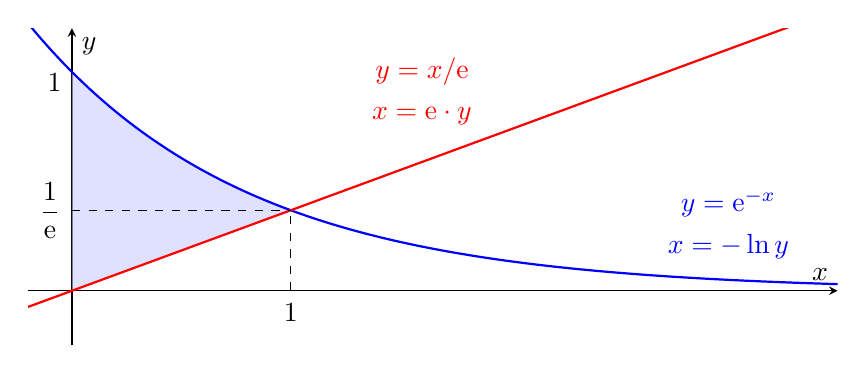
\begin{tikzpicture}
  \begin{axis}[
      axis lines=center,
      axis equal image,
      xlabel={$x$},
      ylabel={$y$},
      ytick=\empty, xtick=\empty,
      xmin=-0.2, xmax=3.5,
      ymin=-0.25, ymax=1.2,
      samples=250,
      clip=true,
      scale=1.5,
      domain=-0.5:4,
    ]

    \addplot [thick, blue, name path=A] {e^(-x)};
    \addplot [thick, red, name path=B] {x/e};
    \addplot [blue!20, fill opacity=0.6] fill between[of=A and B, soft clip={domain=0:1}];
    
    \node at (1,-0.1) {$1$};
    \node at (-0.1,0.367) {$\dfrac1{\mathrm e}$};
    \node at (-0.08,0.95) {$1$};

    \node[red] at (1.6,1) {$y=x/\mathrm{e}$};
    \node[red] at (1.6,0.8) {$x=\mathrm{e}\cdot y$};

    \node[blue] at (3,0.4) {$y=\mathrm{e}^{-x}$};
    \node[blue] at (3,0.2) {$x=-\ln y$};

    \draw[dashed] (0,0.367)--(1,0.367); \draw[dashed] (1,0)--(1,0.367);

  \end{axis}
\end{tikzpicture}
\end{center}

\[V=\int_D2\pi\cdot h(y)\cdot r(y)\,dy=\boxed{\int_0^{1/\mathrm e}2\pi\cdot y\cdot\left(\mathrm e\cdot y-0\right)\,dy+\int_{1/\mathrm e}^12\pi\cdot y\cdot\left(-\ln y-0\right)\,dy}\]

\newpage

\noindent (b)
\begin{center}
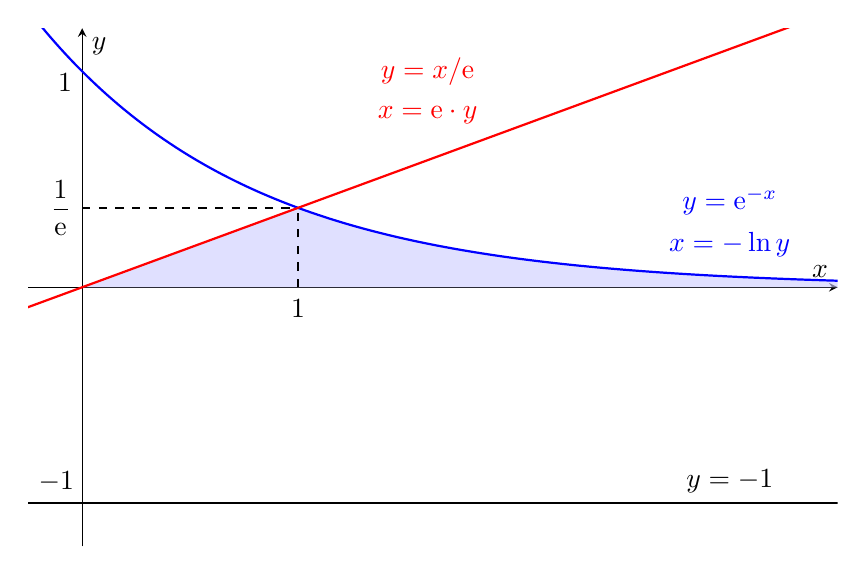
\begin{tikzpicture}
  \begin{axis}[
      axis lines=center,
      axis equal image,
      xlabel={$x$},
      ylabel={$y$},
      ytick=\empty, xtick=\empty,
      xmin=-0.25, xmax=3.5,
      ymin=-1.2, ymax=1.2,
      samples=250,
      clip=true,
      scale=1.5,
      domain=-0.5:4,
    ]

    \addplot [thick, blue, name path=A] {e^(-x)};
    \addplot [thick, red, name path=B] {x/e};
    \addplot [draw=none, name path=C] {0};
    \addplot [blue!20, fill opacity=0.6] fill between[of=B and C, soft clip={domain=0:1}];
    \addplot [blue!20, fill opacity=0.6] fill between[of=A and C, soft clip={domain=1:4}];

    \node at (1,-0.1) {$1$};
    \node at (-0.1,0.367) {$\dfrac1{\mathrm e}$};
    \node at (-0.08,0.95) {$1$};

    \node[red] at (1.6,1) {$y=x/\mathrm{e}$};
    \node[red] at (1.6,0.8) {$x=\mathrm{e}\cdot y$};

    \node[blue] at (3,0.4) {$y=\mathrm{e}^{-x}$};
    \node[blue] at (3,0.2) {$x=-\ln y$};

    \node at (-0.12,-0.9) {$-1$};
    \node at (3,-0.9) {$y=-1$};

    \draw[dashed] (0,0.367)--(1,0.367); \draw[dashed] (1,0)--(1,0.367); \draw[thick] (-1,-1)--(4,-1); 

  \end{axis}
\end{tikzpicture}
\end{center}
\[V=\int_D\pi\left[r_2^2(x)-r_1^2(x)\right]\,dx=\boxed{\int_0^1\left[\left(\frac x{\mathrm e}+1\right)^2-1^2\right]\,dx+\int_1^{\infty}\left[\left(\mathrm{e}^{-x}+1\right)^2-1^2\right]\,dx}\]

\hfill

\noindent (c)
\begin{equation}V=2\pi\left[\int_0^{1/\mathrm e}\mathrm{e}y^2\,dy-\int_{1/\mathrm e}^1y\ln y\,dy\right]\end{equation}

\hfill

\noindent Calculate the integral on the left in $(1)$.

\[\int_0^{1/\mathrm e}\mathrm{e}y^2\,dy=\frac{\mathrm{e}y^3}3\Bigg|_0^{1/\mathrm{e}}=\frac1{3\mathrm{e}^2}\]

\hfill

\noindent Calculate the integral on the right in $(1)$ by using the method of integration by parts.

\[\left.\begin{array}{c}
u=\ln x\implies du=\dfrac1x\,dx\\[1em]
dv=x\,dx\implies\displaystyle v=\frac{x^2}2
\end{array}\right\}\rightarrow\int_a^b u\,dv=uv\bigg|_a^b-\int_a^b v\,du\]

\begin{align*}\int_{1/\mathrm e}^1x\ln x\,dx&=\frac{x^2\ln x}2\Bigg|_{1/\mathrm{e}}^1-\int_{1/\mathrm{e}}^1\frac{x^2}2\cdot\frac1x\,dx=\frac{x^2\ln x}2-\frac{x^2}4\Bigg|_{1/\mathrm{e}}^1\\\\&=\left(0-\frac14\right)-\left(-\frac1{2\mathrm{e}^{2}}-\frac1{4\mathrm{e}^2}\right)=\frac3{4\mathrm{e}^2}-\frac14\end{align*}

\hfill

\noindent Therefore,

\[V=2\pi\left[\left(\frac1{3\mathrm{e}^2}\right)-\left(\frac3{4\mathrm{e}^2}-\frac14\right)\right]=\boxed{\pi\left(\frac12-\frac5{6\mathrm{e}^2}\right)}\]

\newpage

\noindent 3.

\hfill

\noindent (a) Apply the $n$th Term Test for divergence. The inverse trigonometric function $\arctan$ is continuous on $\mathbb{R}$. Therefore, we may take the limit inside the function.

\[\lim_{n\to\infty}\frac1{\arctan\left(n^2\right)}=\frac1{\arctan\left(\displaystyle\lim_{n\to\infty}n^2\right)}=\frac1{\dfrac\pi2}=\frac2\pi\neq1\]

\hfill

\noindent By the $n$th Term Test for divergence, the series $\displaystyle\sum_{n=1}^{\infty}\frac1{\arctan\left(n^2\right)}$ diverges.

\hfill

\hfill

\noindent (b) Recall the sine inequality $-\theta\leq\sin\theta\leq\theta$. Then for all $n\in\mathbb{R}$ except zero, we have $\displaystyle-\frac1{n^3}\leq\sin\left(\frac1{n^3}\right)\leq\frac1{n^3}$. The series $\displaystyle\sum_{n=1}^\infty\frac1{n^3}$ converges because it is a $p$-series with $p=3>1$. By the $p$-series Test, the series converges. The series $\displaystyle\sum_{n=1}^{\infty}\sin\left(\frac1{n^3}\right)$ also converges by the Direct Comparison Test because $\displaystyle\sin\left(\frac1{n^3}\right)<\frac1{n^3}$ for every $n\geq1$.

\hfill

\hfill

\noindent (c) Take $f(x)=x\mathrm{e}^{-x^2}$. $f$ is continuous because the product of a polynomial and an exponential expression is still continuous. $f$ is positive and decreasing for $x\geq1$. Verify the monotonicity of $f$ by taking the first derivative.

\[\frac{df}{dx}=1\cdot\mathrm{e}^{-x^2}+x\mathrm{e}^{-x^2}\cdot(-2x)=\mathrm{e}^{-x^2}\left(1-2x^2\right)\]

\[f'(x)<0\quad\text{for}\quad x>\frac{\sqrt2}2\implies f'(x)<0\quad\text{for}\quad x\geq1\]

\hfill

\noindent We may now apply the Integral Test. Take the limit for the improper integral.

\[\int_1^{\infty}x\mathrm{e}^{-x^2}\,dx=\lim_{R\to\infty}\int_1^Rx\mathrm{e}^{-x^2}\,dx=\lim_{R\to\infty}-\frac12\mathrm{e}^{-x^2}\Bigg|_1^R=\lim_{R\to\infty}-\frac12\left(\mathrm{e}^{-R^2}-\mathrm{e^{-1}}\right)=\frac1{2\mathrm{e}}\]

\hfill

\noindent The integral converges. Then the series $\displaystyle\sum_{n=1}^{\infty}n\mathrm{e}^{-n^2}$ also converges.

\hfill

\noindent 4.

\hfill

\noindent (a) Apply the Ratio Test for absolute convergence, and apply other tests at the endpoints.

\begin{align*}\lim_{n\to\infty}\left|\frac{2^{n+2}\cdot(x+1)^{n+1}}{(n+1)\cdot3^{n+1}}\cdot\frac{n\cdot3^n}{(x+1)^n\cdot2^{n+1}}\right|&=\lim_{n\to\infty}\left|\frac{2n\cdot(x+1)}{(n+1)\cdot3}\right|\\\\&=\frac{2|x+1|}3\cdot\lim_{n\to\infty}\left|\frac{n}{n+1}\right|=\frac{2|x+1|}3\end{align*}
\[\frac{2|x+1|}3<1\implies|x+1|<\frac32\]

\hfill

\noindent The radius of convergence is $\boxed{\dfrac32}$.

\hfill

\[|x+1|<\frac32\implies-\frac32<x+1<\frac32\implies-\frac52<x<\frac12\quad(\text{convergent})\]

\hfill

\noindent Investigate the convergence at the endpoints.

\[x=\frac12\implies\sum_{n=1}^{\infty}\frac{2^{n+1}\cdot\left(\dfrac32\right)^n}{n\cdot3^n}=\sum_{n=1}^{\infty}\frac2n=2\cdot\sum_{n=1}^{\infty}\frac1n\]

\hfill

\noindent This is a $p$-series with $p=1$, for which the series diverges by the $p$-series Test. Try the other endpoint.

\[x=-\frac52\implies\sum_{n=1}^{\infty}\frac{2^{n+1}\cdot\left(-\dfrac32\right)^n}{n\cdot3^n}=\sum_{n=1}^{\infty}\frac{2\cdot(-1)^n}n=2\cdot\sum_{n=1}^{\infty}\frac{(-1)^n}n\]

\hfill

\noindent This is an alternating series. The non-alternating part, which is $\frac1n$, is nonincreasing for $n\geq1$ and it is positive. The limit at infinity is $0$. By Leibniz's Alternating Series Test, the series converges.

\noindent The convergence set for the power series is $\boxed{\left[-\dfrac52,\dfrac12\right)}$.

\hfill

\noindent (b)
\begin{align*}f(x)&=\frac{x^{123}}{1+x^4}=x^{123}\cdot\frac1{1-\left(-x^4\right)}=x^{123}\cdot\sum_{n=0}^{\infty}\left(-x^4\right)=x^{123}\cdot\sum_{n=0}^{\infty}(-1)^n\cdot x^{4n}\\\\&=\boxed{\sum_{n=0}^{\infty}(-1)^n\cdot x^{123+4n}=x^{123}-x^{127}+x^{131}-x^{135}+...}\end{align*}

\end{document}